\documentclass[UTF8]{ctexart}   
\usepackage{amsmath} % 提供数学符号支持
\usepackage{amssymb} % 提供更多数学符号支持
\usepackage{graphicx} % 用于插入图片
\usepackage[a6paper,centering,scale=0.8]{geometry} % 用于设置页面边距
\usepackage{float}
% 定义一个新的引用环境,使用楷体和小五号字体(修正:补全右花括号)
\newenvironment{myquote}{\begin{quote}\kaishu\zihao{-5}}{\end{quote}} 

% 定义定理环境
\newtheorem{thm}{定理} 

% 定义新命令(如果不需要可以删除)
\newcommand\degree{^\circ}

\begin{document}
\pagestyle{plain}
\title{\heiti 杂谈勾股定理\thanks{省教育厅项目资助}} % 标题
\author{\kaishu 李汉龙 \thanks {沈阳建筑大学理学院}
\and \kaishu 隋英 \thanks {沈阳建筑大学理学院}
\and \kaishu 韩婷  \thanks{沈阳电视大学文法学院}}
\date{\today} % 日期
\maketitle % 生成标题
\listoftables % 显示所有表格标签
\begin{abstract}
    这是一篇关于勾股定理的小短文。其中内容可能包含文字、公式、图形、表格等。
\end{abstract}

\tableofcontents % 生成目录

\section{勾股定理在古代}  
\label{sec:ancient}
西方称勾股定理为毕达哥拉斯定理,将勾股定理的发现归功于公元前6世纪
的毕达哥拉斯学派\cite{Kline}。该学派得到了一个法则,可以求出可排成直角
三角形三边的三元数组。毕达哥拉斯学派没有书面著作,该定理的严格表述和证明
则见于欧几里得\footnote{欧几里得,公元前 330-275 年。}《几何原本》的命题 
47:“直角三角形斜边上的正方形等于两直角边上的两个正方形之和。”证明是用面积
做的。\par    %\par 命令用于显式开始一个新段落

我国《周髀算经》载商高(约公元前12世纪)答周公问:
\begin{myquote}  
勾广三,股修四,径隅五。
\end{myquote}

又载陈子(公元前7--6世纪)答荣方向:
\begin{myquote}
若求邪至日者,以日下为勾,日高为股,勾股各自乘,并而开方除之,得邪至日。
\end{myquote}  

都较古希腊更早,后者已经明确指出勾股定理的一般形式。图\ref{fig:xiantu} 是我国古代对勾股定理的一种证明\cite{quanjing}。


\begin{figure}[H]%强制在当前位置插入图片
    \centering
    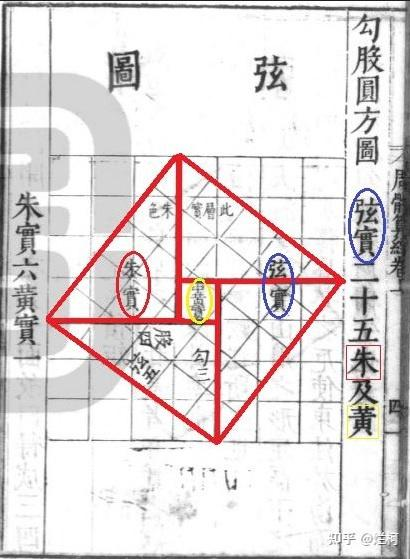
\includegraphics[scale=0.5]{xiantu.png} % 插入图形,缩小0.5,缩放系数为0.5
    \caption{\zihao{-5}\kaishu 宋赵爽在《周髀算经》中做的弦图(仿制),该图给出了勾股定理的一个极具对称美的证明。\label{fig:xiantu}}
\end{figure}

\section{勾股定理的近代形式}

% 使用标准的 equation 环境(或自定义 equationl)
\begin{thm}[勾股定理] 

直角三角形斜边的平方等于两腰的平方和。
\par 可以用符号语言表述为:设直角三角形 $ABC$,其中 $\angle C = 90^\circ$,则有
\begin{equation} % 改用标准 equation 环境
\label{eq:gougu}
AB^2 = BC^2 + AC^2.
\end{equation}
\end{thm}

满足式 \eqref{eq:gougu} 的整数称为\emph{勾股数}。第 \ref{sec:ancient} 节所说毕达哥拉斯学派得到的三元数组就是勾股数。下表列出一些较小的勾股数:
%\emph这个语法默认效果:将文本显示为斜体(italic),用于突出关键术语、定义或需要读者注意的部分
\vspace{3mm}

\begin{tabular}{|c|c|c|} \hline
直角边 $a$ & 直角边 $b$ & 斜边 $c$ \\ \hline
3 & 4 & 5 \\ \hline
5 & 12 & 13 \\ \hline
\end{tabular}

$(a^2 + b^2 = c^2)$ % 行内公式

\begin{thebibliography}{99}
\bibitem{1} 矢野健太郎. 几何的有名定理. 上海科学技术出版社, 1986.
\bibitem{quanjing} 曲安金. 商高、赵爽与刘徽关于勾股定理的证明. 数学传播, 20(3), 1998.
\bibitem{Kline} 克莱因. 古今数学思想. 上海科学技术出版社, 2002.
\end{thebibliography}

\addcontentsline{toc}{section}{参考文献}

\begin{appendix}
\section{附录}
勾股定理又叫商高定理,国外也称百牛定理。
\end{appendix}

\end{document}